
%%--------------------------------------------------
%% Holt: Multiple Choice Questions
%%--------------------------------------------------


%% Chapter 03: Two Dimensional Motion and Vectors
%%--------------------------------------------------


%% Holt Multiple Choice Questions
%%--------------------------------------------------
\element{holt-mc}{
\begin{question}{holt-ch03-Q01}
    Vector $\mathbf{A}$ has magnitude of 30 units.
    Vector $\mathbf{B}$ is perpendicular to vector $\mathbf{A}$ and has a magnitude of 40 units.
    What would the magnitude of the resultant vector $\mathbf{A} + \mathbf{B}$ be?
    \begin{multicols}{2}
    \begin{choices}
        \wrongchoice{10 units}
      \correctchoice{50 units}
        \wrongchoice{70 units}
        \wrongchoice{zero}
    \end{choices}
    \end{multicols}
\end{question}
}

\element{holt-mc}{
\begin{question}{holt-ch03-Q02}
    What term represents the magnitude of a velocity vector?
    \begin{multicols}{2}
    \begin{choices}
        \wrongchoice{acceleration}
        \wrongchoice{momentum}
      \correctchoice{speed}
        \wrongchoice{velocity}
    \end{choices}
    \end{multicols}
\end{question}
}

\newcommand{\HoltChThreeQThree}{
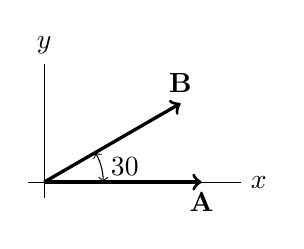
\begin{tikzpicture}
    %% X and Y axis
    \draw (-0.2,0) -- (2.5,0) node[anchor=west] {$x$};
    \draw (0,-0.2) -- (0,1.5) node[anchor=south] {$y$};
    %% vectors
    \draw[very thick,->] (0,0) -- ++ (0:2) node[anchor=north] {$\mathbf{A}$};
    \draw[very thick,->] (0,0) -- ++ (30:2) node[anchor=south] {$\mathbf{B}$};
    %% vectors
    \draw[<->] (0:0.75) arc (0:30:0.75) node[pos=0.5,anchor=west]{\ang{30}};
\end{tikzpicture}
}

\element{holt-mc}{
\begin{question}{holt-ch03-Q03-A}
    Two vectors, $\mathbf{A}$ and $\mathbf{B}$,
        are graphically represented.
    \begin{center}
        \HoltChThreeQThree
    \end{center}
    What is the direction of the resultant vector $\mathbf{A}+\mathbf{B}$?
    \begin{choices}
      \correctchoice{\ang{15} above the $x$-axis}
        \wrongchoice{\ang{75} above the $x$-axis}
        \wrongchoice{\ang{15} below the $x$-axis}
        \wrongchoice{\ang{75} below the $x$-axis}
    \end{choices}
\end{question}
}

\element{holt-mc}{
\begin{question}{holt-ch03-Q03-B}
    Two vectors, $\mathbf{A}$ and $\mathbf{B}$,
        are graphically represented.
    \begin{center}
        \HoltChThreeQThree
    \end{center}
    What is the direction of the resultant vector $\mathbf{B}+\mathbf{A}$?
    \begin{choices}
        \wrongchoice{\ang{15} left of the $y$-axis}
        \wrongchoice{\ang{75} left of the $y$-axis}
        \wrongchoice{\ang{15} right of the $y$-axis}
      \correctchoice{\ang{75} right of the $y$-axis}
    \end{choices}
\end{question}
}

\element{holt-mc}{
\begin{question}{holt-ch03-Q04-A}
    Two vectors, $\mathbf{A}$ and $\mathbf{B}$,
        are graphically represented.
    \begin{center}
        \HoltChThreeQThree
    \end{center}
    What is the direction of the resultant vector $\mathbf{A}-\mathbf{B}$?
    \begin{choices}
        \wrongchoice{\ang{15} above the $x$-axis}
        \wrongchoice{\ang{75} above the $x$-axis}
        \wrongchoice{\ang{15} below the $x$-axis}
      \correctchoice{\ang{75} below the $x$-axis}
    \end{choices}
\end{question}
}

\element{holt-mc}{
\begin{question}{holt-ch03-Q04-B}
    Two vectors, $\mathbf{A}$ and $\mathbf{B}$,
        are graphically represented.
    \begin{center}
        \HoltChThreeQThree
    \end{center}
    What is the direction of the resultant vector $\mathbf{B}-\mathbf{A}$?
    \begin{choices}
      \correctchoice{\ang{15} left of the $y$-axis}
        \wrongchoice{\ang{75} left of the $y$-axis}
        \wrongchoice{\ang{15} right of the $y$-axis}
        \wrongchoice{\ang{75} right of the $y$-axis}
    \end{choices}
\end{question}
}

\element{holt-mc}{
\begin{question}{holt-ch03-Q05}
    A motorboat heads due east at \SI{5.0}{\meter\per\second}
        across a river that flows towards the south at a speed of \SI{5.0}{\meter\per\second}.
    What is the resultant velocity relative to an observer on the shore?
    \begin{choices}
        \wrongchoice{\SI{3.2}{\meter\per\second} to the southeast}
        \wrongchoice{\SI{5.0}{\meter\per\second} to the southeast}
      \correctchoice{\SI{7.1}{\meter\per\second} to the southeast}
        \wrongchoice{\SI{10.0}{\meter\per\second} to the southeast}
    \end{choices}
\end{question}
}

\element{holt-mc}{
\begin{question}{holt-ch03-Q06}
    A motorboat heads due east at \SI{5.0}{\meter\per\second}
        across a river that flows towards the south at a speed of \SI{5.0}{\meter\per\second}.
    If the river is \SI{125}{\meter} wide,
        how long does the boat take to cross the river?
    \begin{multicols}{2}
    \begin{choices}
        \wrongchoice{\SI{39}{\second}}
      \correctchoice{\SI{25}{\second}}
        \wrongchoice{\SI{17}{\second}}
        \wrongchoice{\SI{12}{\second}}
    \end{choices}
    \end{multicols}
\end{question}
}

\element{holt-mc}{
\begin{question}{holt-ch03-Q07}
    The pilot of a plane measures an air velocity of \SI{165}{\kilo\meter\per\hour} south relative to the plane.
    An observer on the ground sees the plan pass overhead at a velocity of \SI{145}{\kilo\meter\per\hour} toward the north.
    What is the velocity of the wind that is affecting the plane relative to the observer?
    \begin{multicols}{2}
    \begin{choices}
        \wrongchoice{\SI{20}{\kilo\meter\per\hour} to the north}
      \correctchoice{\SI{20}{\kilo\meter\per\hour} to the south}
        \wrongchoice{\SI{165}{\kilo\meter\per\hour} to the north}
        \wrongchoice{\SI{310}{\kilo\meter\per\hour} to the south}
    \end{choices}
    \end{multicols}
\end{question}
}

\element{holt-mc}{
\begin{question}{holt-ch03-Q08}
    A golfer takes two putts to sink his ball in the hole once he is on the green.
    The first putt displaces the ball \SI{6.00}{\meter} east,
        and the second putt displaces the ball \SI{5.40}{\meter} south.
    What displacement would put the ball in the hole in one putt?
    \begin{choices}
        \wrongchoice{\SI{11.40}{\meter} southeast}
        \wrongchoice{\SI{8.07}{\meter} at \ang{48} south of east}
        \wrongchoice{\SI{3.32}{\meter} at \ang{42} south of east}
      \correctchoice{\SI{8.07}{\meter} at \ang{42} south of east}
    \end{choices}
\end{question}
}

\element{holt-mc}{
\begin{question}{holt-ch03-Q09}
    A girl riding a bicycle at \SI{2.0}{\meter\per\second} throws a tennis ball horizontally forward at a speed of \SI{1.0}{\meter\per\second} from a height of \SI{1.5}{\meter}.
    At the same moment, a boy standing on the sidewalk drops a tennis ball straight down from a height of \SI{1.5}{\meter}.
    What is the initial speed of the girl's ball relative to the boy?
    \begin{multicols}{2}
    \begin{choices}
        \wrongchoice{\SI{1.0}{\meter\per\second}}
        \wrongchoice{\SI{1.5}{\meter\per\second}}
        \wrongchoice{\SI{2.0}{\meter\per\second}}
      \correctchoice{\SI{3.0}{\meter\per\second}}
    \end{choices}
    \end{multicols}
\end{question}
}

\element{holt-mc}{
\begin{question}{holt-ch03-Q10}
    A girl riding a bicycle at \SI{2.0}{\meter\per\second} throws a tennis ball horizontally forward at a speed of \SI{1.0}{\meter\per\second} from a height of \SI{1.5}{\meter}.
    At the same moment, a boy standing on the sidewalk drops a tennis ball straight down from a height of \SI{1.5}{\meter}.
    If air resistance is disregarded, which ball will hit the ground first?
    \begin{multicols}{2}
    \begin{choices}
        \wrongchoice{the boy's ball}
        \wrongchoice{the girl's ball}
      \correctchoice{both at the same time}
        \wrongchoice{The answer cannot be determined from the given information}
    \end{choices}
    \end{multicols}
\end{question}
}

\element{holt-mc}{
\begin{question}{holt-ch03-Q11}
    A girl riding a bicycle at \SI{2.0}{\meter\per\second} throws a tennis ball horizontally forward at a speed of \SI{1.0}{\meter\per\second} from a height of \SI{1.5}{\meter}.
    At the same moment, a boy standing on the sidewalk drops a tennis ball straight down from a height of \SI{1.5}{\meter}.
    If air resistance is disregarded,
        which ball will have the greater speed (relative to the ground) when it hits the ground?
    \begin{multicols}{2}
    \begin{choices}
        \wrongchoice{the boy's ball}
      \correctchoice{the girl's ball}
        \wrongchoice{neither}
        \wrongchoice{The answer cannot be determined from the given information}
    \end{choices}
    \end{multicols}
\end{question}
}

\element{holt-mc}{
\begin{question}{holt-ch03-Q12}
    A girl riding a bicycle at \SI{2.0}{\meter\per\second} throws a tennis ball horizontally forward at a speed of \SI{1.0}{\meter\per\second} from a height of \SI{1.5}{\meter}.
    At the same moment, a boy standing on the sidewalk drops a tennis ball straight down from a height of \SI{1.5}{\meter}.
    What is the speed of the girl's ball when it hits the ground?
    \begin{multicols}{2}
    \begin{choices}
        \wrongchoice{\SI{1.0}{\meter\per\second}}
        \wrongchoice{\SI{3.0}{\meter\per\second}}
      \correctchoice{\SI{6.2}{\meter\per\second}}
        \wrongchoice{\SI{8.4}{\meter\per\second}}
    \end{choices}
    \end{multicols}
\end{question}
}


\endinput

